% Póster científico vertical, Evidencia 1 (MA2015.201).
% Compilar desde esta carpeta:
%   TECTONIC_CACHE_DIR=/tmp/tectonic-cache /tmp/tectonic-bin/tectonic poster.tex
% Apellidos: completar en \author si hacen falta.
\PassOptionsToPackage{table}{xcolor}
\documentclass[final]{beamer}

\usepackage[orientation=portrait,size=a0,scale=1.0]{beamerposter}
\usetheme{default}

\usepackage[spanish,es-tabla,es-noshorthands]{babel}
\spanishplainpercent
\usepackage[utf8]{inputenc}
\usepackage[T1]{fontenc}
\usepackage{lmodern}
\usepackage{amsmath,amssymb}
\usepackage{booktabs}
\usepackage{graphicx}
\usepackage{array}

\graphicspath{{../figures/}}

\definecolor{navy}{HTML}{041E42}
\definecolor{blue}{HTML}{0B4F9E}
\definecolor{bright}{HTML}{1565C0}
\definecolor{ice}{HTML}{E7F1FB}
\definecolor{paper}{HTML}{FFFFFF}
\definecolor{gain}{HTML}{D3E6FA}
\definecolor{ink}{HTML}{0E1C2F}

\setbeamercolor{background canvas}{bg=ice}
\setbeamercolor{headline}{fg=white,bg=navy}
\setbeamercolor{finding}{fg=white,bg=bright}
\setbeamercolor{footline}{fg=white,bg=navy}
\setbeamercolor{block title}{fg=white,bg=blue}
\setbeamercolor{block body}{fg=ink,bg=paper}
\setbeamercolor{normal text}{fg=ink,bg=ice}

\setbeamerfont{title}{series=\bfseries,size=\VeryHuge}
\setbeamerfont{author}{size=\Large}
\setbeamerfont{institute}{size=\large}
\setbeamerfont{block title}{series=\bfseries,size=\large}
\setbeamerfont{block body}{size=\normalsize}
\setbeamerfont{footline}{size=\footnotesize}

\setbeamertemplate{navigation symbols}{}
\setbeamertemplate{itemize item}{\raise1.2pt\hbox{\color{bright}\rule{1.8mm}{1.8mm}}}
\setlength{\leftmargini}{1.15em}
\setlength{\itemsep}{0.22em}
\setlength{\parsep}{0pt}
\setlength{\parskip}{0.28em}

\setbeamertemplate{headline}{%
  \begin{beamercolorbox}[wd=\paperwidth,leftskip=1.4cm,rightskip=1.4cm,sep=2.6mm]{headline}
    \vspace{1mm}
    {\usebeamerfont{title}%
      Selección evolutiva de portafolios en mercados reales:\par
      \vspace{1.2mm}%
      réplica y mejora híbrida\par}
    \vspace{1.8mm}
    {\usebeamerfont{author}\insertauthor\par}
    \vspace{0.8mm}
    {\usebeamerfont{institute}\insertinstitute\par}
    \vspace{0.6mm}
  \end{beamercolorbox}%
  \begin{beamercolorbox}[wd=\paperwidth,leftskip=1.4cm,rightskip=1.4cm,sep=2.4mm]{finding}
    \textbf{Hallazgo.}
    Elegir los activos con un algoritmo evolutivo y sus pesos con programación cuadrática mejora el frente de Pareto en las 12 instancias.
    Fuera de muestra, en 2024, el Sharpe mediano cae de alrededor de 2{,}7 a 0{,}3--0{,}5 y esa ventaja desaparece.
  \end{beamercolorbox}%
}

\setbeamertemplate{footline}{%
  \begin{beamercolorbox}[wd=\paperwidth,leftskip=1.3cm,rightskip=1.3cm,sep=2.2mm]{footline}
    \textbf{Referencias.}\;
    [1] Hidalgo-Marín, A.\,J.; Nebro, A.\,J.; García-Nieto, J.
    Efficient selection of investment portfolios in real-world markets: A multi-objective optimization approach.
    \textit{Algorithms} \textbf{2026}, \textit{19}, 20.
    \texttt{doi:10.3390/a19010020}.\;
    [2] López de Prado, M. Building diversified portfolios that outperform out of sample.
    \textit{J. Portfolio Management} \textbf{2016}, \textit{42}(4), 59--69.\;
    [3] Blank, J.; Deb, K. pymoo.
    \textit{IEEE Access} \textbf{2020}, \textit{8}, 89497--89509.\;
    [4] Deb et al., \textit{IEEE TEVC} \textbf{2002} (NSGA-II);
    Zhang y Li, \textit{IEEE TEVC} \textbf{2007} (MOEA/D);
    Beume, Naujoks y Emmerich, \textit{EJOR} \textbf{2007} (SMS-EMOA).\;
    [5] Goldfarb e Idnani, \textit{Math. Programming} \textbf{1983} (QP).
  \end{beamercolorbox}%
}

\title{Selección evolutiva de portafolios en mercados reales: réplica y mejora híbrida}
\author{Eduardo \texorpdfstring{\quad\textperiodcentered\quad}{ y }Juan Pedro}
\institute{Tecnológico de Monterrey \quad MA2015.201 \quad Agosto--diciembre 2026}

\begin{document}
\begin{frame}[t]
\vspace{2.5mm}

\begin{columns}[t,onlytextwidth]
\begin{column}{0.488\textwidth}
\begin{block}{Problema y formulación}
Réplica de Hidalgo-Marín, Nebro y García-Nieto [1]: cartera de cardinalidad fija sobre mercados estadounidenses de 2023. Dos objetivos, ambos a minimizar,
\[
f_1=\sqrt{250\,w^{\top}\Sigma_{S}w},
\qquad
f_2=-\sum_{j\in S}w_{j}R_{j}.
\]
\(S\) tiene \(k\) activos, \(\sum_{i\in S} w_i=1\) y cada peso vive en \(\bigl[\tfrac{1}{2k},\tfrac{2}{k}\bigr]\). El riesgo es la volatilidad anualizada, la cantidad de las figuras del artículo.

Doce instancias: siete de \(k=5\) sobre 100 activos (NYSE, NASDAQ, OTC, AMEX, ARCA, BATS y ALL) y cinco de \(k=20\) (ALL con 100, 500, 1\,000, 3\,000 y 6\,000 activos). Presupuesto: 50\,000 evaluaciones, \(\times 2\) a \(\times 5\) en los universos grandes.

Se replican el orden de los algoritmos (IGD+ e hipervolumen), los diagramas de diferencia crítica y la forma de los frentes, más las carteras de las tablas 8 a 14.
\end{block}
\end{column}
\begin{column}{0.012\textwidth}\end{column}
\begin{column}{0.488\textwidth}
\begin{block}{Algoritmo y metodología}
La solución tiene \(2k\) genes, no \(2N\): \(k\) punteros de activo y \(k\) pesos. El activo es \(\lfloor s_{i}N\rfloor\); si ya está tomado, pasa al siguiente índice libre. Los pesos se normalizan y se proyectan al intervalo. Operadores de la tabla 3, en pymoo [3]: población 100, SBX (\(p_{c}=0{,}9\), \(\eta=20\)), mutación polinomial (\(p_{m}=1/n\), \(\eta=20\)). MOEA/D usa PBI (\(\theta=5\)), \(T=20\) y a lo más \(n_{r}=2\) reemplazos. SMS-EMOA es de estado estacionario.

10 corridas por algoritmo e instancia (el artículo usa 30), semillas 12345 a 12354. IGD+ e hipervolumen se normalizan con el ideal y el nadir; el punto de referencia del HV es \((1{,}1,\ 1{,}1)\). Entre variantes, Wilcoxon de rangos al 5\,\% sobre la mediana de cada corrida. Entre algoritmos, Friedman y Nemenyi.

Python, pymoo, NumPy y el QP de Goldfarb--Idnani [5]. Cada corrida se guarda al terminar. En 6 núcleos la réplica tardó 63 min.

\begin{center}
\footnotesize
\setlength{\tabcolsep}{3.5pt}
\renewcommand{\arraystretch}{1.08}
\begin{tabular}{@{}>{\raggedright\arraybackslash}p{0.16\linewidth}>{\raggedright\arraybackslash}p{0.40\linewidth}>{\raggedright\arraybackslash}p{0.36\linewidth}@{}}
\toprule
& \textbf{Activos} & \textbf{Pesos} \\
\midrule
Réplica & punteros reales, sondeo lineal & SBX y mutación; luego se acotan \\
HRP & conjunto de \(k\) ids, cruce por ranura & igual que la réplica \\
Híbrido & igual que HRP, orden de hojas & QP exacta y un gen de intercambio \\
\bottomrule
\end{tabular}
\end{center}
\end{block}
\end{column}
\end{columns}

\vspace{2.2mm}
\begin{block}{Mejora propuesta}
El evolutivo solo elige los \(k\) activos; los pesos salen de un QP convexo [5]. Un gen \(t\in[0,1]\) recorre esa frontera, con aversión \(\gamma=10^{-2+6t}\). Si dos genes repiten un activo, el duplicado sigue el orden de hojas de López de Prado [2]: en ALL\(_{20}\) de 6\,000 nombres ese vecino correlaciona 0{,}56, frente a 0{,}48 de la réplica.

\vspace{1.4mm}
\begin{center}
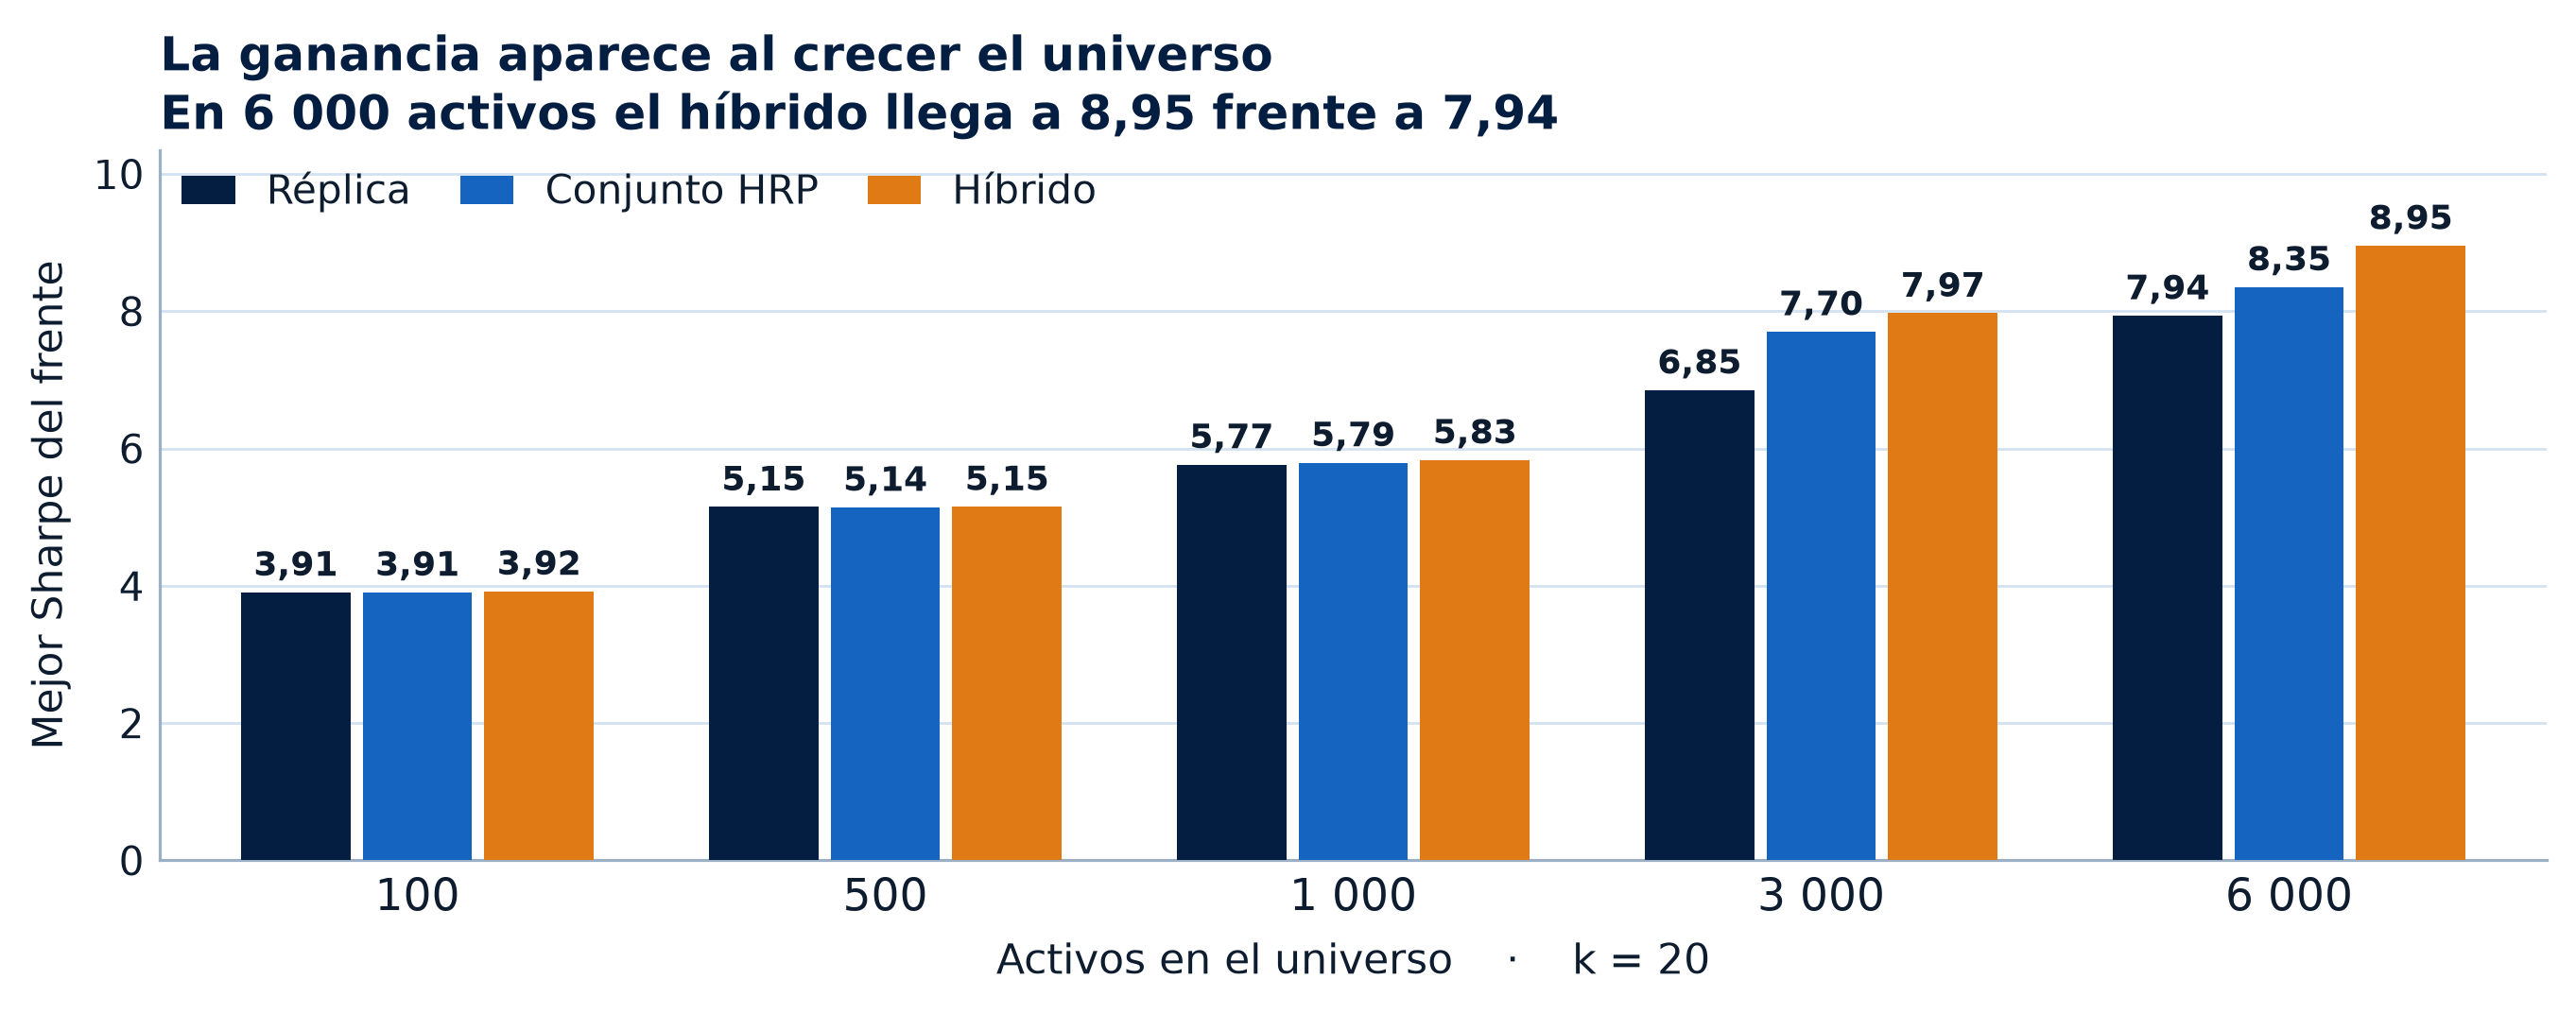
\includegraphics[width=0.96\linewidth]{poster_sharpe_k20.png}
\end{center}
{\footnotesize
Mejor Sharpe del frente de referencia, \(SR=(R-R_{f})/\sigma\), \(R_{f}=6{,}97\,\%\).
En \(k=5\) las tres variantes coinciden a menos de 0{,}005.
El híbrido tiene el mejor HV e IGD+ en las 12 instancias y supera a la réplica en 33 de 36 pares (Wilcoxon, 5\,\%).
\par}
\end{block}

\vspace{2.0mm}
\begin{columns}[t,onlytextwidth]
\begin{column}{0.488\textwidth}
\begin{block}{Réplica frente al artículo}
\begin{center}
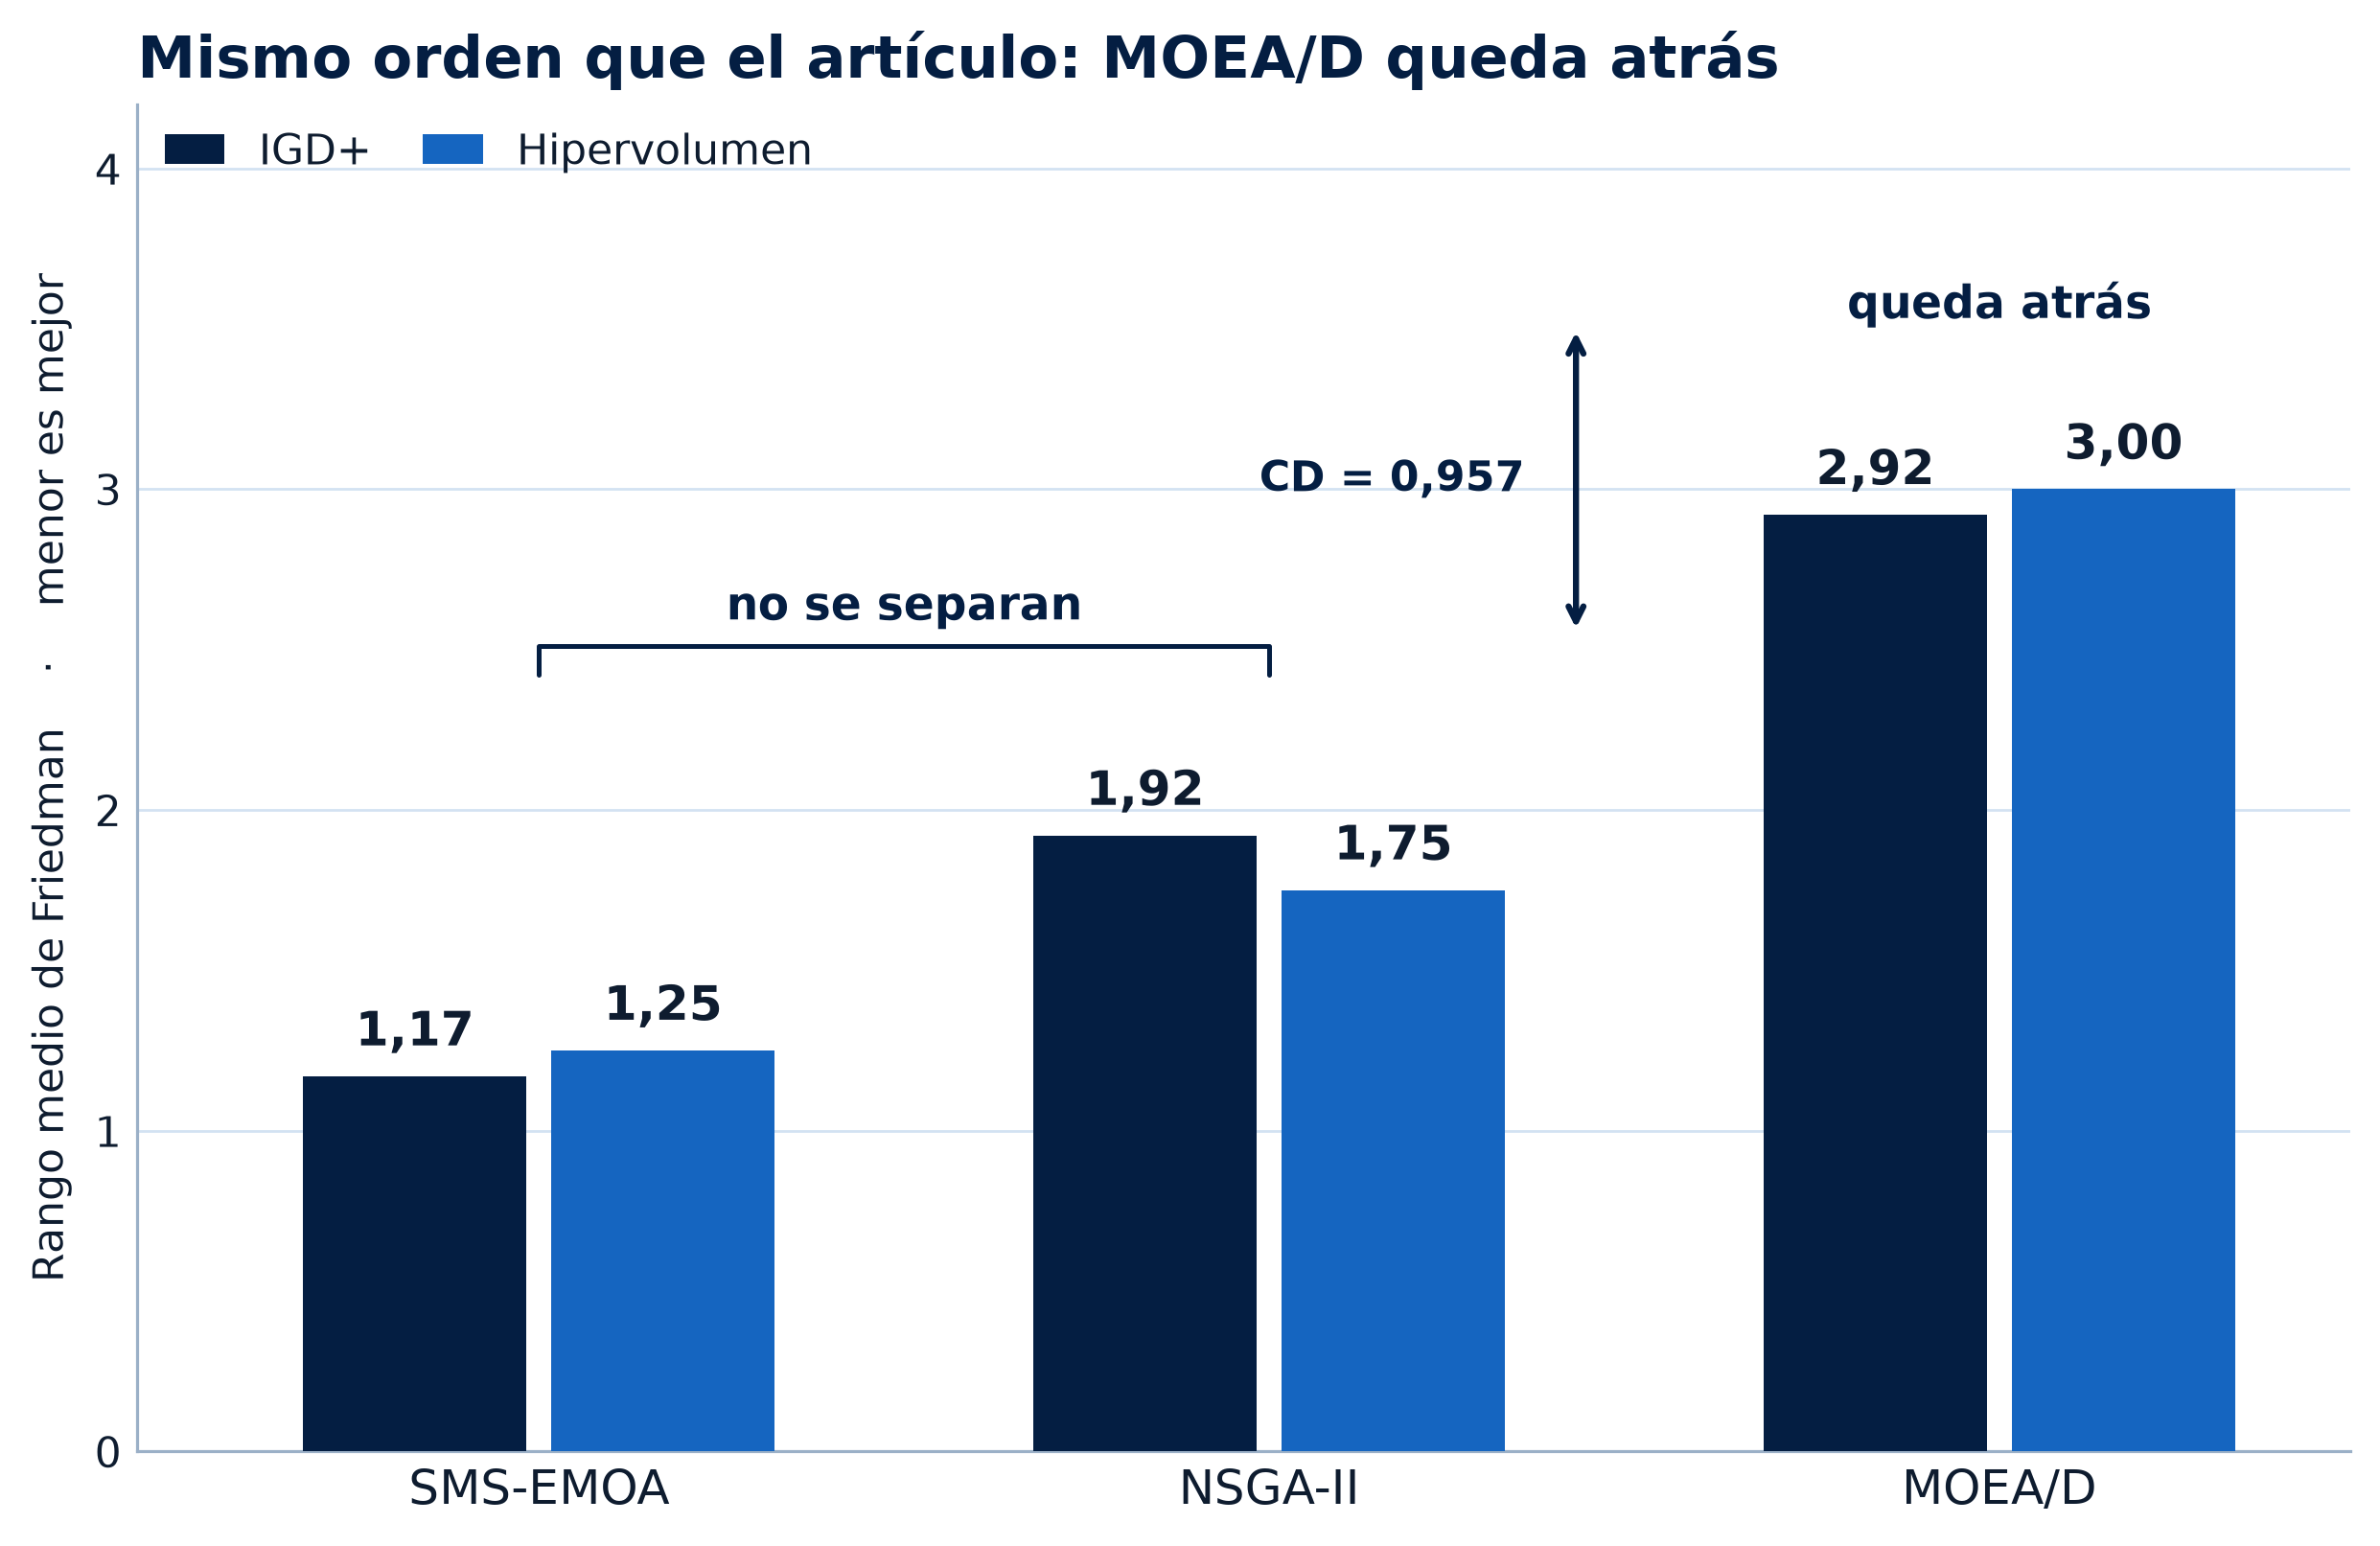
\includegraphics[width=\linewidth]{poster_ranks.png}
\end{center}
{\footnotesize
Rango medio de Friedman, 12 instancias. Nemenyi, \(\alpha=0{,}05\), CD\({}=0{,}957\).
\par}
\vspace{1.0mm}
\begin{itemize}
\item SMS-EMOA lidera el IGD+ en 10 de 12 instancias y el hipervolumen en 9. En BATS de 5 activos aporta el 65\,\% del frente.
\item ALL de 20 activos y 6\,000 nombres: retorno máximo cercano a 218\,\% con riesgo 66--68\,\% (artículo: 218{,}85\,\% y 67{,}89\,\%).
\item MOEA/D se queda en el centro. En AMEX su frente mediano arranca en riesgo \(\approx 0{,}09\); el de referencia, en \(0{,}05\).
\end{itemize}
\end{block}
\end{column}
\begin{column}{0.012\textwidth}\end{column}
\begin{column}{0.488\textwidth}
\begin{block}{Fuera de muestra, 2024}
Los frentes se optimizaron con precios de 2023. El año 2024 sale de Yahoo Finance. Entra una cartera si al menos el 80\,\% de su peso tiene historia completa en ambos años: 926 de 1\,266 tickers.
\vspace{1.2mm}
\begin{center}
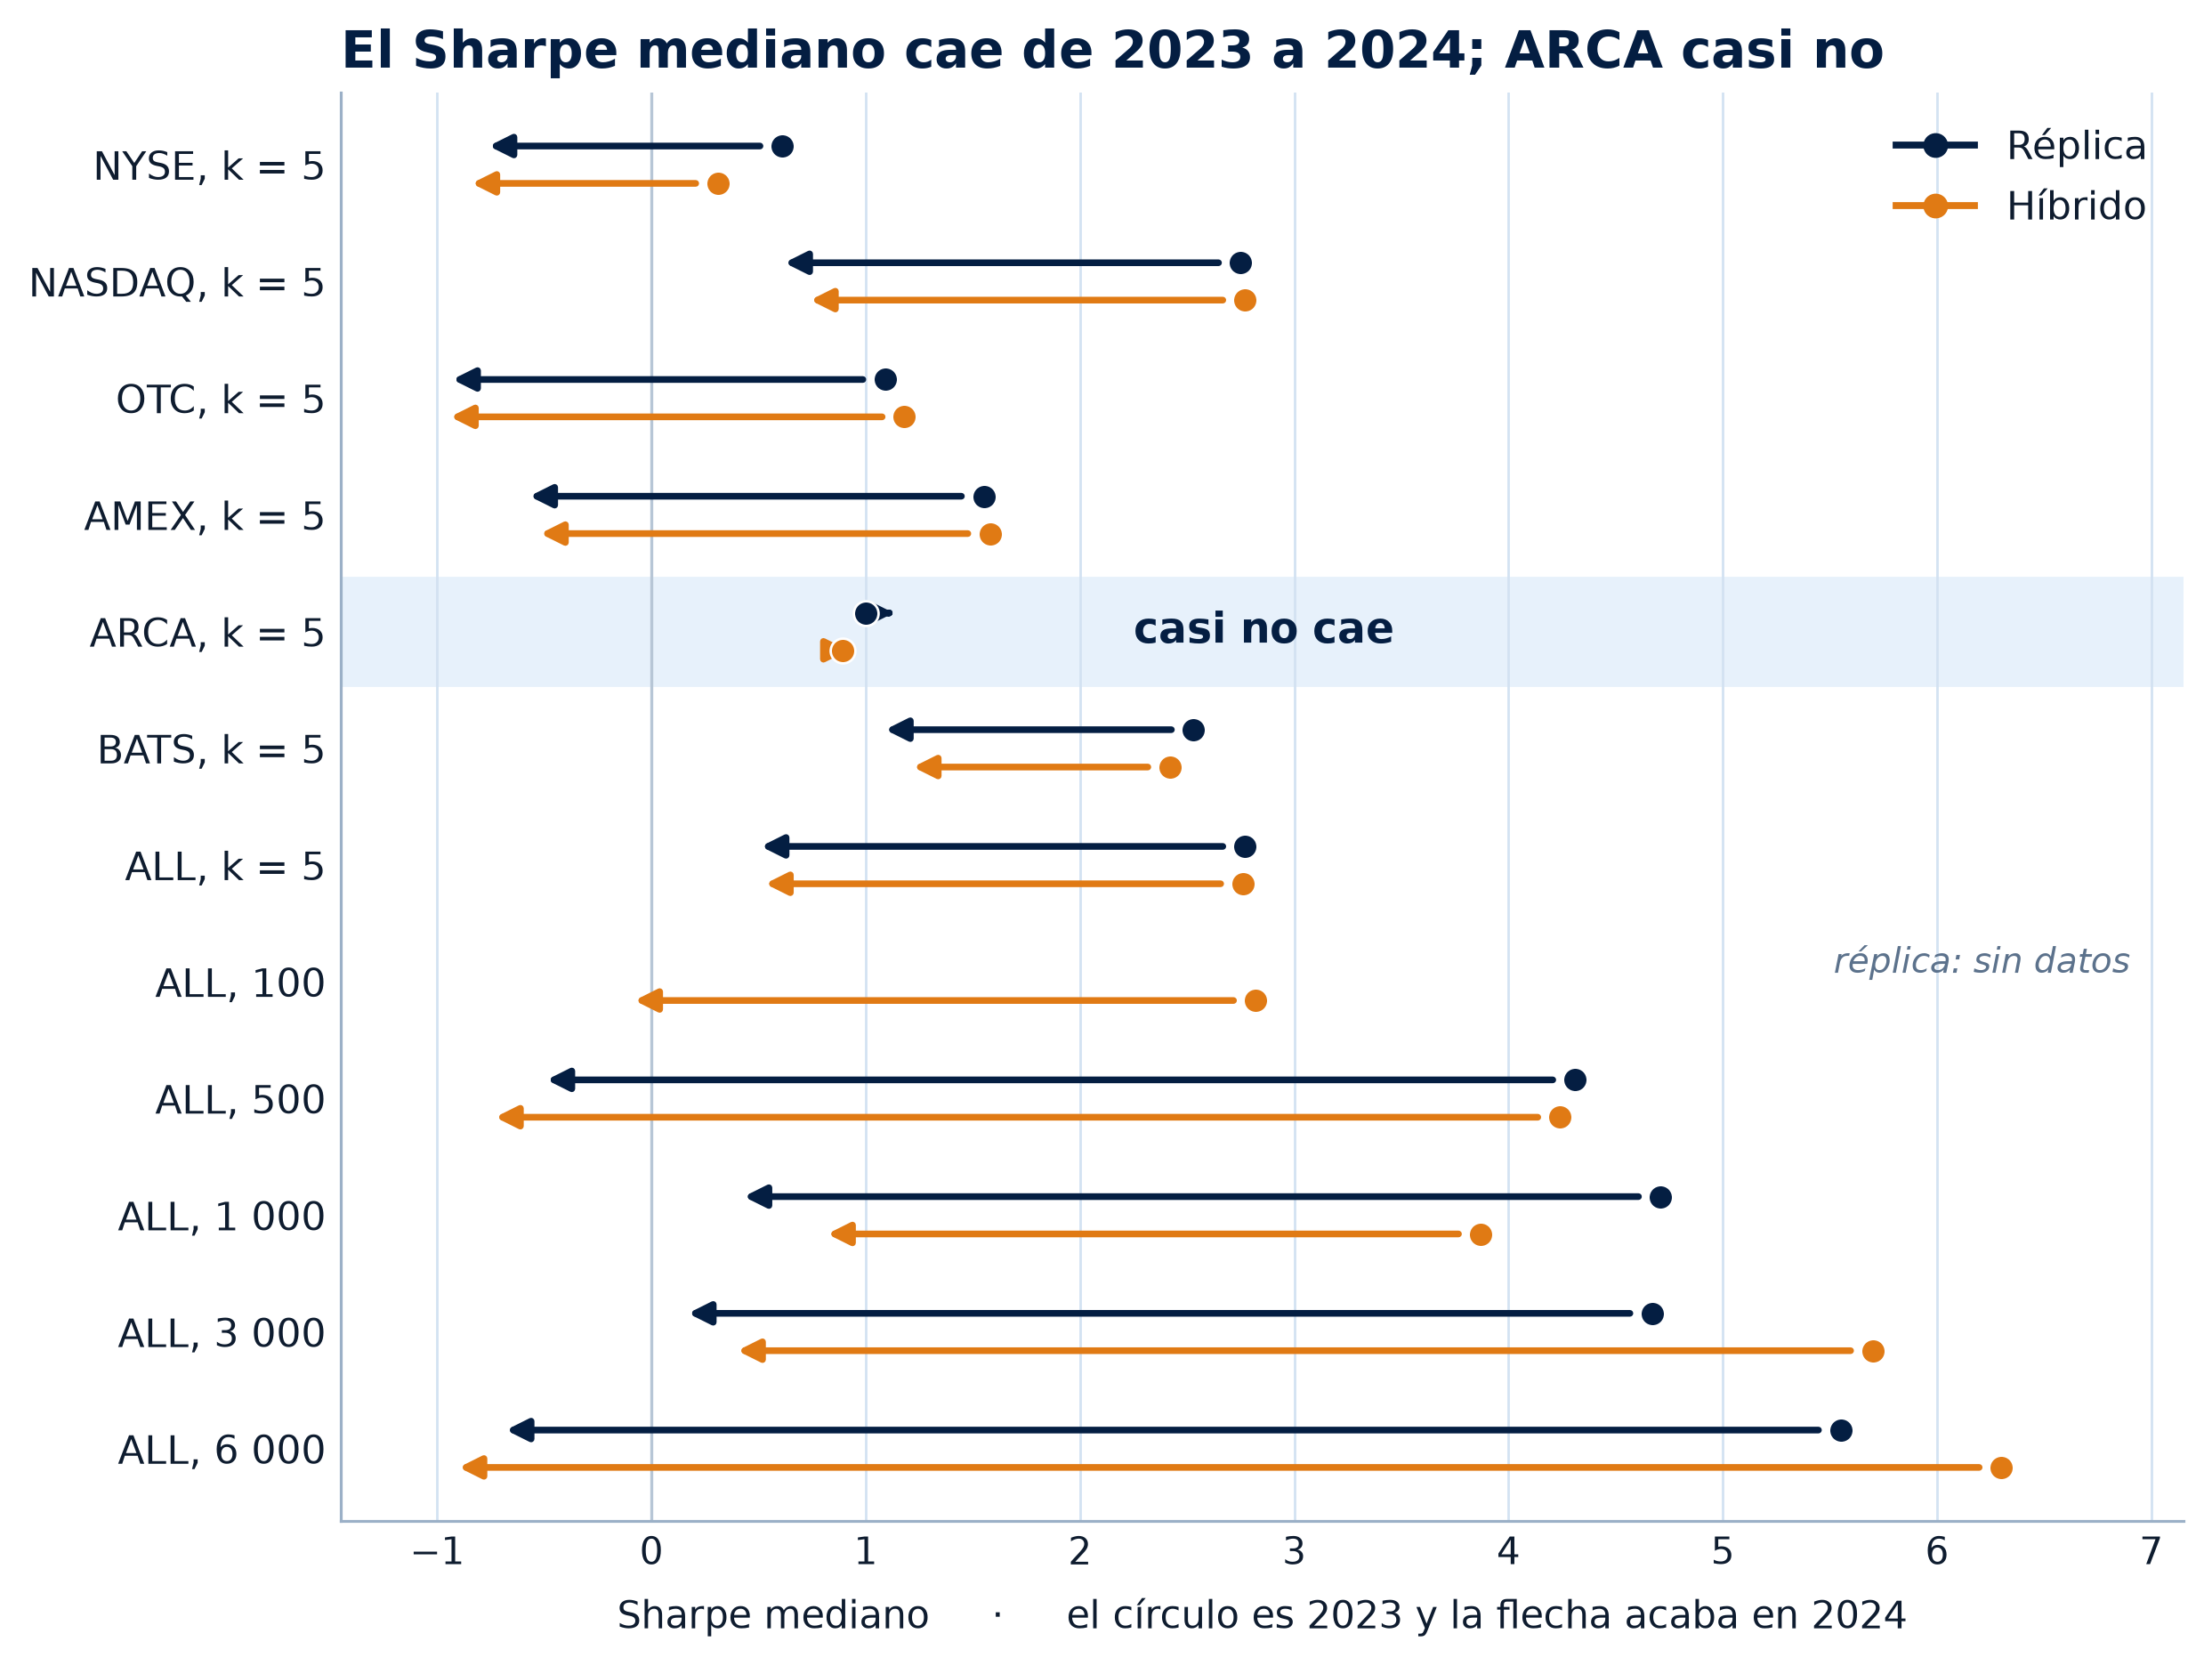
\includegraphics[width=\linewidth]{poster_oos_sharpe.png}
\end{center}
{\footnotesize
Cada flecha va del Sharpe mediano de 2023 al de 2024.
ALL\(_{20}\) de 100 activos, réplica: sin carteras evaluadas.
\par}
\end{block}
\end{column}
\end{columns}

\vspace{1.4mm}
\begin{block}{Conclusiones}
\begin{columns}[t,onlytextwidth]
\begin{column}{0.32\textwidth}
\textbf{Comportamiento.}
SMS-EMOA cubre mejor el frente; NSGA-II lo sigue; MOEA/D se concentra en el centro. Con \(k=5\) evolucionar los pesos es fácil. Con \(k=20\) es el cuello de botella, y el QP devuelve un punto eficiente para que el evolutivo busque la combinación de activos.
\end{column}
\begin{column}{0.34\textwidth}
\textbf{Replicabilidad.}
El orden estadístico, la forma de los frentes y las carteras representativas se recuperan. En el código, y no en el texto: la codificación es \(2k\), el riesgo graficado es volatilidad anualizada, y \textit{Fitness} es \((R-R_{f})/\sqrt{\text{riesgo}}\), no el Sharpe de libro. El artículo incluye SMPSO; esta réplica no. Aquí hay 10 corridas, no 30.
\end{column}
\begin{column}{0.32\textwidth}
\textbf{Fuera de muestra.}
El Sharpe mediano pasa de 2{,}7 en 2023 a 0{,}3--0{,}5 en 2024 (cambio \(\approx -2{,}2\)). Cae en 97--100\,\% de las carteras, salvo ARCA. El híbrido gana en 6 de 11 instancias y pierde en 5. Parte del hueco ya está en series rotas de 2023; el resto es que un año de retornos no pronostica el siguiente.
\end{column}
\end{columns}
\end{block}

\end{frame}
\end{document}
